\documentclass[10pt,a4paper]{article}
\usepackage[utf8]{inputenc}
\usepackage{amsmath}
\usepackage{amsfonts}
\usepackage{amssymb}
\usepackage{hyperref}
\usepackage{listings}
\usepackage[many]{tcolorbox}
\tcbuselibrary{listings}

\newtcblisting{mylisting}{
  listing only,
  hbox,
  colframe=cyan,
  colback=cyan!10,
  listing options={
    language=Fortran,
    basicstyle=\small\ttfamily,
    breaklines=true,
    columns=fullflexible
  },
}

%hyperlink parameters
\hypersetup{
    colorlinks=true,
    linkcolor=blue,
    filecolor=magenta,      
    urlcolor=cyan,
    pdftitle={Overleaf Example},
    pdfpagemode=FullScreen,
    }
\urlstyle{same}

% Code style font
\usepackage{xcolor}
\definecolor{light-gray}{gray}{0.95}
\newcommand{\code}[1]{\colorbox{light-gray}{\texttt{#1}}}
%\newcommand{\code}{\texttt}

% Fortran source code style



\author{Sarah}
\title{Guide: How to work with PGI on Colab}
%\date{today}

\begin{document}
\maketitle{}
\newpage

\section{Introduction}
This document will summerize how to install the PGI compilers on Colab.\\
Before going further, make sure you have a Google account and that your drive is quite empty (you will need the maximum space as possible). Storage limitation is an important part to handle to success installing PGI compilers using Colab.\\

\section{Before installation}
\subsection{Downloading the package}
The first step consist in download the package from your \textbf{local machine}. To do so, execute the following command on your terminal, as follow:\\
{\small \code{\$ wget https:\/\/developer.download.nvidia.com\/hpc\-sdk\/22.11\/nvhpc\_2022\_2211\_Linux\_x86\_64\_cuda\_11.8.tar.gz}}\\
\subsection{Upload the file on the Drive}
Once the file is downloaded in your current directory, you can open your \textit{drive} and select \textit{New} \\
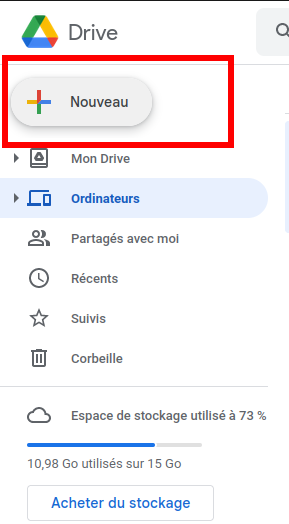
\includegraphics[scale=0.4]{newfile.png}\\
Then, select \textit{Import a file}:\\
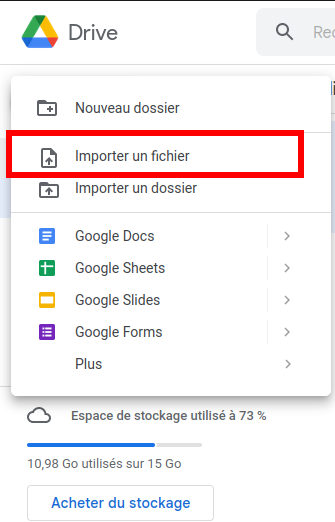
\includegraphics[scale=0.4]{importfile.png}\\
You only need to select the directory where you stored the compressed file (\code{*.tar.gz}).\\
This operation could take few minutes or maybe an hour depending your internet connection speed.\\

\subsection{Extract the archive}
Now that we have our compressed file stored in our drive, we can proceed the next steps on Colab.\\
To do that, we need to open a new Colaboroty file. You can do that from your \textit{drive menu} and select \textit{New} as seen previously and then select Google Colaboratory\\
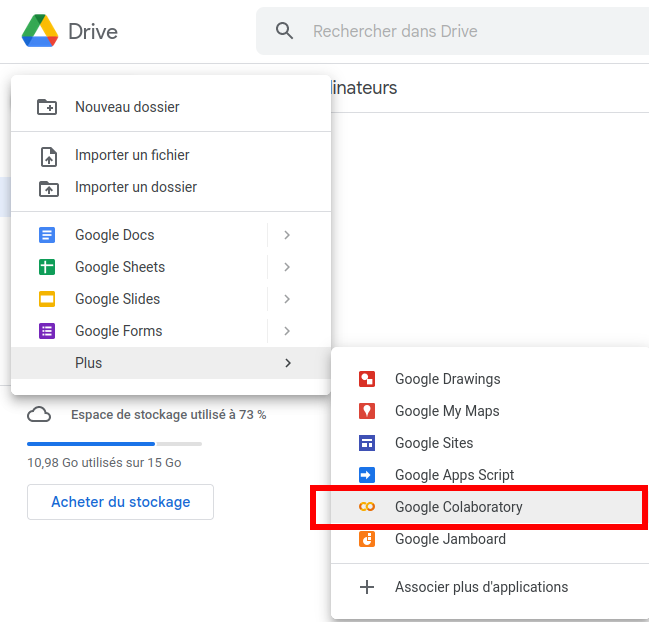
\includegraphics[scale=0.4]{newColab.png}\\

\subsection{Change the Runtime}
You are now using the Colab notebook, and before going further, it is important to change the runtime type first and foremost. This needs to be at the beginning of your work session, otherwise you will lose your session and start again from the beginning. The installation of the PGI compilers is part of a more extented work which aim to port a code to GPUs. Actually, strictly speaking, the installation does not require to work on a GPU Runtime session, but later on, we will test the \code{-acc} flag to compile a code. So it is better to get into the habit of enabling GPU.\\
To do that, select in the menu \textbf{Runtime}, then select \textbf{Change runtime type}, you will have the following menu\\
\begin{center}
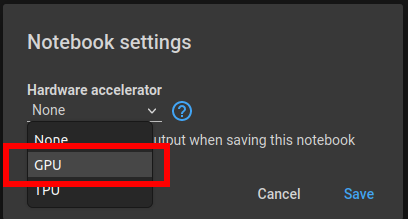
\includegraphics[scale=0.4]{gputype.png}
\end{center}
Choose the \textbf{GPU} type and save the changes.\\

\subsection{Import the file from the Drive}
At this stage, our content (the compressed file) is stored on the Drive, and we are working on Colab. It is important to highlight the fact Colab is made for interactive use only, it is not meant to store data permanently. For this reason, we have to import our data from the Drive as follow\\
\begin{center}
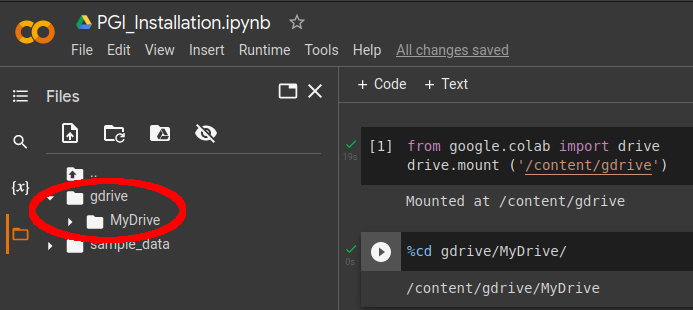
\includegraphics[scale=0.4]{mountdrive.png}
\end{center}
This allows us now to get access to the Drive content during our work session. We assume that you uploaded the \code{*.tar.gz} file in the main menu of the Drive. If it is the case, you can find then the file in the following directory \code{/content/gdrive/MyDrive}.
\subsection{Extract the archive}
Execute the following command on the Colab notebook:\\
\code{\$ !tar -xvf nvhpc\_2022\_2211\_Linux\_x86\_64\_cuda\_11.8.tar.gz --remove-files} \\
The  \code{--remove-files} option allow you remove the compressed file after the extraction. Indeed, we will recall the importance of the storage capacity in your Drive, since we are working with big files. So make sure, to empty your Drive after the installation. Removing the compressed file is not sufficient. You will need to get access to the storage management in this \href{https:\/\/one.google.com\/storage\/management}{link} and make sure the recycle bin is empty.\\
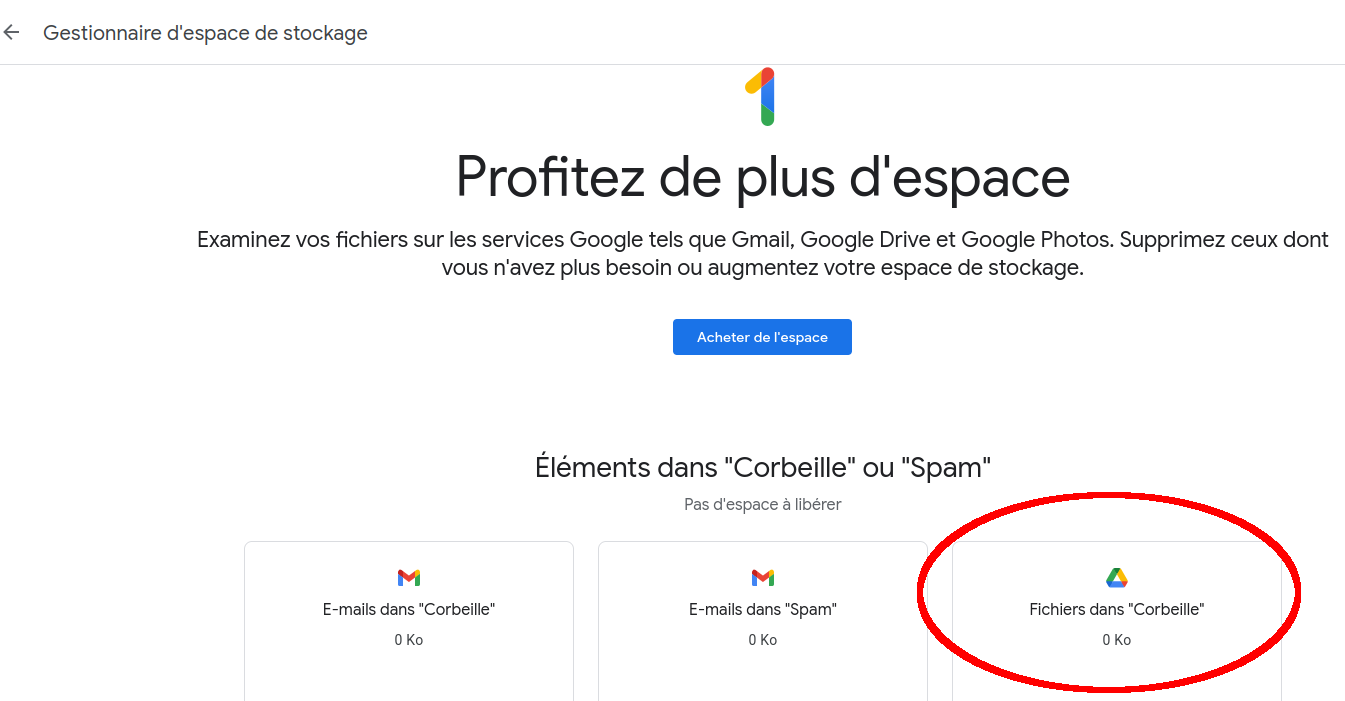
\includegraphics[scale=0.3]{freestorage.png}\\
You should have now the folder \code{nvhpc\_2022\_2211\_Linux\_x86\_64\_cuda\_11.8} in your Drive.

\section{Installation}
All the installation  will be done in our Colab notebook. At this stage, your folder \code{nvhpc\_2022\_2211\_Linux\_x86\_64\_cuda\_11.8} may not appear from your Colab notebook. You can just execute again the first command to update your Drive content. Then we will change directory to get access to the \code{install} file by these two commands:\\
\code{\$ \%cd nvhpc\_2022\_2211\_Linux\_x86\_64\_cuda\_11.8}\\
\code{\$ \%cd install\_components/}\\
\subsection{Launching installation}
Now, we can launch the installation by executing this command:\\
\code{\$ !./install -b}\\
The \code{-b} option is necesserary as it will allow to keep an interactive mode during the installation, in particular when it comes to press the \textit{Enter key} or change the installation directory.
\begin{center}
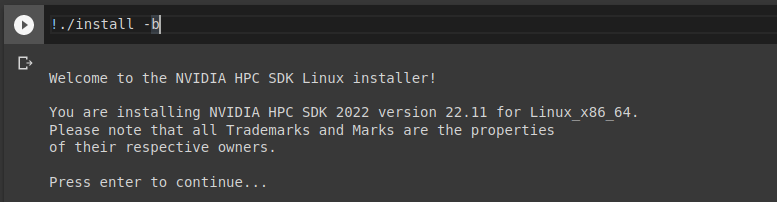
\includegraphics[scale=0.4]{install_1.png}
\end{center}
After this message, you have to drag the pointer right below this sentence and click, and then press \textit{Enter}.\\
After, you will be asked to choose an install option, just press \textit{Enter} again
\begin{center}
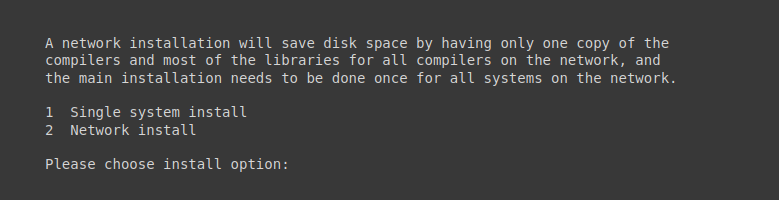
\includegraphics[scale=0.4]{install_2.png}
\end{center}

\subsection{Installation directory}
At this stage, we will recall the interactive mode specific to Colab. Indeed, there is nothing relevant at choosing the default path proposed during the installation, since it is rooted in the short-lived folders of Colab. So, as a workaround we will create (\code{mkdir}) a new folder in our Drive. We can call it \code{nvhpc} ; therefore you can  enter the path \code{/content/gdrive/MyDrive/nvhpc} the when asking and then press \textit{Enter}
\begin{center}
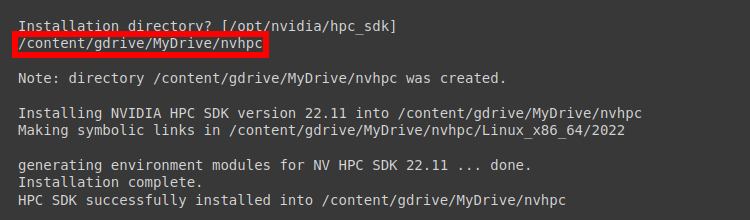
\includegraphics[scale=0.4]{install_3.png}
\end{center}
The installation will take few minutes to complete.

\vspace{0.2cm}
\textbf{IMPORTANT:} Again, you should remove now the folder \code{nvhpc\_2022\_2211\_Linux\_x86\_64\_cuda\_11.8} and then clean it from the storage management it as seen above.\\

\subsection{PATH setting}
To use the HPC SDK, we need to initialize the shell variables and create new paths.\\
\underline{For the \code{MANPATH}}\\
\code{\$ import os}\\
\code{\$ os.environ['MANPATH'] = ":/content/gdrive/MyDrive/nvhpc/Linux\_x86\_64/22.11/compilers/man"}\\
\vspace{0.2cm}\\
\underline{For the \code{PATH}}\\
\code{\$ import os}\\
\code{\$ os.environ['PATH'] += ":/content/gdrive/MyDrive/nvhpc/Linux\_x86\_64/22.11/compilers/bin"}\\
We can check the values of the environment variables by executing the following commands:\\
\code{\$ !\$PATH}
\code{\$ !\$MANPATH}

\vspace{0.2cm}
\textbf{IMPORTANT:} These setting have to be done everytime we start a new session.\\

\subsection{Permissions}
Now, the package HPC SDK has been successfully installed into the Drive into \code{/content/gdrive/MyDrive/nvhpc}.\\
As we noticed when we wanted to import content from the Drive into the Colab notebook, we had to give permissions to get access to our Google account.\\
In the same way, we have to change the permission attributes related to our folder containing our compilers by doing so\\
\code{\$ !chmod -R 777 /content/gdrive/MyDrive/nvhpc/Linux\_x86\_64/22.11/}


\end{document}